\subsection{QCDCL}

In this section, we will present an algorithm that can solve a QBF instance, with the underlying proof of the solution given in the Q-Resolution framework. The quantified conflict driven clause learning is the quantified version for the CDCL used for SAT solving. For the propositional problem in the satisfiable case it's enough to have an assignment, thus the CDCL algorithm tries to guess an assignment that evaluates the input to true, but in case the decisions result in a false formula, the procedure tries to derive a clause that minimize the search space. Similarly, in QCDCL we learn clauses to prune the search space of falsifying assignments, and learn cubes for running the satisfying assignment, \cite{handbook}.

\textrosu{Propozitie sa introduc ce urmeaza.}

\begin{figure}[H]
\centering
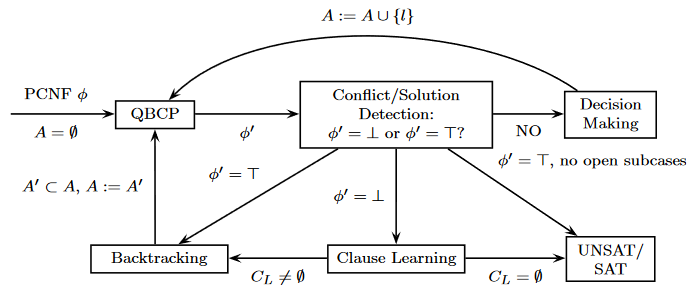
\includegraphics[width=1\textwidth]{../graphics/qcdcl-flowchart.png}
\caption{Flowchart of QCDCL from \cite{handbook}.}
\end{figure}

\stodo{cum merge figura}

\begin{definition}[Unit literal detection \cite{handbook}]
    A clause $C \in \phi$ is \textbf{unit} iff $C$ contains one literal, and the literal is existential quantified. That literal is also called a \textbf{unit literal}. \textbf{Unit literal detection} applied to a QBF collects all unit clauses in the QBF.
\end{definition}

\begin{example}
    Let our formula be $\forall x_1x_2 \exists y_1 \forall x_3 \exists y_2 (x_1 \lor x_2) \land x_3 \land y_1 \land \overline{y_2}$. The unit literal detection gives us $\{y_1, \overline{y_2}\}$.
\end{example}

\begin{definition}[QBCP \cite{handbook}]
    Given a PCNF $\phi$ and the empty assignment $A = \{\}$. We apply the following:
    \begin{enumerate}
        \item Apply universal reduction (UR) on $\phi[A]$ to get $\phi[A]'$.
        \item Apply unit literal detection (UL) on $\phi[A]$ and append the result to $A$.
        \item Repeat from 1. Stop if $A$ haven't changed, or the formula is true or false.
    \end{enumerate}
\end{definition}

\begin{example}\label{example:qbcp}
    Given $\phi = \forall x_1 x_2 \exists y (x_1 \lor x_2 \lor \overline{y}) \land (y \lor \overline{x_1}) \land (y \lor \overline{x_y}) \land y$ we apply QBCP, we start with $A$ empty:
    \begin{itemize}
        \item We cannot apply UR.
        \item From $\phi[]$ with UL, we get $A = \{ y \}$.
        \item $\phi[y] = \forall x_1 x_2 (x_1 \lor x_2)$, we apply UR on $x_2$, and we get $\phi[y] = x_1$
        \item We cannot apply UL, because no existential literal is present.
        \item By applying UR, we get $\phi[y] = \bot$. Thus, we stop.
    \end{itemize}
\end{example}

\stodo{the scope of the work is not the solver but to derive a prove briefly bla bla}
Using the previous example \ref{example:qbcp}, 

\textrosu{how a proof would look like for $\exists xy (\neg x \lor y)$ after assign of $x$}